%!TEX root = ../../main.tex
\section{Projektgennemførelse}
\subsection{Specificering af projektet}
Katrines Kælder på Ingeniørhøjskolen i Århus, havde lavet et opslag om at de manglede et kasseapparat. Her var der beskrevet krav til produktet og givet en beskrivelse af hvad de forventede. Ud fra kravende blev der opstillet nogle Use Cases så der kom en helt klar afgrænsning om hvad systemmet skal være i stand til når det er færdigt.
\newline
\newline
For at give en bedre afgrænsning af krav til produktet er der blevet brugt MoSCoW-metoden. Ved hjælp af denne er der blevet sat nogle funktionelle og ikke-funktionelle krav.  


\subsection{Arbejdsmetode}
Arbejdet med projektet er gjort rent iterativt og med SCRUM som inspireret  udviklingsproces, i den forstand at der er blevet arbejdet i sprint af to uger ad gangen. I disse sprint er der blevet fastlagt arbejdsopgaver på et scrumboard som derefter blev tildelt til folk i projektgruppen. Opgaverne blev rykke rundt på scrumboarded alt efter om de var tildelt, klar til review, færdig, osv. 
\newline
\newline
Alle dele af projektet er blevet lavet i små dele, hvor de har kunne spille sammen til en vis forstand så der hele tiden har været en smule sammenhold i projektet. 

\begin{figure}[H]
	\centering
	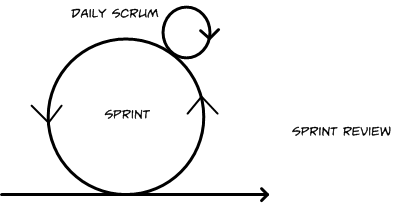
\includegraphics[scale=0.6]{Rapport/sprint_loop_events.PNG}
	\caption{sprint event}
	\label{fig:sprint}
\end{figure} 

\subsection{Proces}
Processen i dette semester projekt har været agil og, som nævnt tidligere, med Scrum som inspirerende udviklingsproces.
\newline
\newline
De fleste dage blev der afholdt et dagligt scrum møde, hvor der er blevet talt om hvilke arbejdsopgaver der er blevet udført og hvilke der mangler. I starten af semesteret blev daily SCRUM udført ca. hver anden dag, mens der senere på semestret blev afholdt et møde hver dag. 


